% ここはもっと分野外の人にもわかるような、基本的・概要的な事項から
% 書き始めましょう。

% あと最後に、先行研究 (Olling & Dehnen 2002; Bovy 2017; Vickers & Smith 2018など) で
% 何がどこまでわかっていて、何がわかっていないのかを書いて、
% それを踏まえて、今回の修論の研究のポイントとの違いをしっかり書かないとダメです。
% これが「研究動機」になるはずです。

\chapter{研究背景}
\section{歴史的流れ}
\section{現状・課題点} % 研究のIntroduction (研究背景・基本事項)、定性的に書く (定量的な事は2章で)
\section{研究の動機}
天の川銀河の中の太陽系の運動速度と方向は、ある程度の値は制限されている。太陽系の運動は通常LSR(Local Standard of Rest)に対する運動で表される。LSRに対する方向は、銀河中心向きのベクトル、銀河回転方向のベクトル、銀北極方向のベクトルを足したような方向である。銀河回転天の川銀河の力学と運動学を研究する上で、太陽運動が必要になるため、太陽運動の測定は天の川銀河研究において重要である。運動の方向については先述した通りであるが、速度についてはまだ銀河回転方向の速度の不定性が大きい。

100年以上の間、天の川銀河の構造を推測するために太陽近傍星の空間分布と動力学が研究されてきた。\cite{Kapteyn1920}は天の川銀河の大きさと厚さを決定するために星の数を使用した。さらに、銀河円盤に対して垂直な方向で静水圧平衡であると仮定することで、視線速度と固有運動から\cite{Kapteyn1922}は初めて天の川銀河の質量の妥当な値を得ることに成功した。しかしながら、\cite{Oort1927a}はKapteynの銀河の質量は球状星団とRR Lyrae星を銀河系に束縛するのに十分な大きさでないと指摘した。\cite{Lindblad1927}は高速度星と球状星団の下位構造はもちろん近傍の低速度星の下位構造も同様に同じ対称軸と共通の中心ー球状星団の下位構造(\cite{Shapley1918})ーを持っていると提案した。Lindbladはさらに、当時の利用可能なデータから、これらのそれぞれの下位構造は力学平衡であり、もっとも大きい回転をする下位構造は最も平坦な空間分布と最も小さな特異運動(\cite{Jeans1922})を持っているという仮説を提唱した。


太陽近傍の星の運動は系統(平均)運動にランダム運動を足したものとして解釈される。円盤銀河では、系統運動がランダム運動に比べて支配的である。そのような恒星系は力学的に冷たいと言われる。例えば、太陽近傍では円盤面の速度分散すなわちランダム運動の大きさは古い星の恒星円盤では$45\mathrm{km\ s^{-1}}$、誕生初期の星では$18\mathrm{km\ s^{-1}}$である一方、系統運動は$200\mathrm{km\ s^{-1}}$のオーダーである。ランダム運動が消える力学的に冷たい極限では、系統運動は重力ポテンシャルによって生まれる閉じた軌道に沿ったものになる。したがって、天の川銀河のポテンシャルと質量分布の知見は恒星系の系統運動の研究から得ることができる。

Oortは彼の先駆的な論文(\cite{Oort1927a})でこの方法の理論的な基礎をまとめた。まず、Oortに従い全ての星が閉じた軌道で運動しているような冷たい系を考える。Oortは実際に天の川銀河を軸対称と考えたが、彼の分析は容易に非軸対称なものに一般化された(\cite{Ogrodnikoff1932}, \cite{Milne1935}, \cite{Chandra42})。

その後、いくつかの先行研究によって太陽運動(太陽の特異運動)が求められてきた。表\ref{table2},\ref{table3}、図\ref{fig:uvw}はそれぞれの先行研究で得られたこれらの値である。\cite{Delhaye1965}は異なるスペクトル型と光度の集団を調べることによって太陽運動を$(U_{\odot},V_{\odot},W_{\odot})=(9,12,7)\ km\ s^{-1}$程度とした。これは3つとも現在でも使用される値である。ここで、$(U_{\odot},V_{\odot},W_{\odot})$はそれぞれ太陽から銀河中心に向かう方向、太陽の銀河回転方向かつ$U_{\odot}$に垂直な方向、銀北極方向のLSRに対する太陽の速度である。

ある集団の星のランダム運動はそれらの年齢、色、金属量、スケールハイト (scale height)の強い関数である。\cite{DB1998}はStr\"{o}mbergのasymmetric drift関係(後述)を用いることで$Hipparcos$のデータから$(U_{\odot},V_{\odot},W_{\odot}) = (10.0, 5.2, 7.2)\ \mathrm{km\ s^{-1}}$ と測定した。
$U_{\odot}, W_{\odot}$については彼らの30年以上前に導かれたDelhayeの値とほぼ同じ値となっている。$V_{\odot}$については後にDelhayeの値と近い値に修正された(\cite{Schonrich2010})。\cite{Schonrich2010}はStr\"{o}mbergの線形関係は円盤の金属量勾配によって無効になることを示した。

\definecolor{Gray}{gray}{0.9}
\definecolor{LightCyan}{rgb}{0.88,1,1}
\def\arraybackslash{\let\\\tabularnewline}

\begin{table}
\begin{center}
%\scalebox{0.5}
\scriptsize
%\footnotesize
%\small
\begin{tabular}{l|l|l|c|c|c|c} \hline
 \rowcolor{LightCyan}
 Label & Reference & Source & $A$ & $B$ & $C$ & $K$\\
  \hline
 \multirow{2}{*}{VS18} & \multirow{2}{*}{\cite{VM2018}$^1$} & RAVE, LAMOST, & \multirow{2}{*}{14.3} & \multirow{2}{*}{-6.7} & \multirow{2}{*}{0.2} & \multirow{2}{*}{-4.5} 
    \\ && TGAS, 若い星 &&&& \tabularnewline[\doublerulesep] 
 \hline
 \multirow{2}{*}{VS18} & \multirow{2}{*}{\cite{VM2018}$^2$} & RAVE, LAMOST, & \multirow{2}{*}{18.8} & \multirow{2}{*}{-12.7} & \multirow{2}{*}{1.7} & \multirow{2}{*}{-7.6} 
    \\ && TGAS, 中間の星 &&&& \tabularnewline[\doublerulesep] 
 \hline
 \multirow{2}{*}{VS18} & \multirow{2}{*}{\cite{VM2018}$^3$} & RAVE, LAMOST & \multirow{2}{*}{17.0} & \multirow{2}{*}{-2.1} & \multirow{2}{*}{8.3} & \multirow{2}{*}{-5.6}
    \\ && TGAS, 古い星 &&&& \tabularnewline[\doublerulesep]
 \hline
 \multirow{2}{*}{Bv17} & \multirow{2}{*}{\cite{Bovy17}} & Gaia DR1 & \multirow{2}{*}{$15.3\pm0.4$} & \multirow{2}{*}{$-11.9\pm0.4$} & \multirow{2}{*}{$-3.2\pm0.4$} & \multirow{2}{*}{$-3.3\pm0.6$}
    \\ && 主系列星 &&&& \tabularnewline[\doublerulesep]
 \hline
 OD03 & \cite{OD03} & ATC / Tycho-2 & 16 & -17 & -10 & -\\
  \hline
\end{tabular}
\caption{オールト定数の先行研究の値をまとめた表。定数$A,B,C,K$の単位は$\mathrm{km\ s^{-1}kpc^{-1}}$。}
\label{table2}
\end{center}
\end{table}

\begin{table}
\begin{center}
%\scalebox{0.5}
%\scriptsize
\footnotesize
%\small
\begin{tabular}{l|l|l|c|c|c} \hline
 \rowcolor{LightCyan}
 Label & Reference & Source & $u_0 \ (\mathrm{km\ s^{-1}})$ & $v_0 \ (\mathrm{km\ s^{-1}})$ & $w_0 \ (\mathrm{km\ s^{-1}})$\\
  \hline
  K19 & \cite{Kawata2019} & Gaia DR2 & $7.7\pm0.9$ & $12.4\pm0.7$ & -\\ 
  \hline
  H15 & \cite{Huang2015} & LSS-GAC DR1 & $7.01\pm0.20$ & $10.13\pm0.12$ & $4.95\pm0.09$\\ 
  \hline
  BB14 & \cite{Bobylev2014} & 若い星 & $6.00\pm0.50$ & $10.60\pm0.80$ & $6.50\pm0.30$\\ 
  \hline
  C11 & \cite{Coskunoglu2011} & RAVE DR3 & $8.50\pm0.29$ & $13.38\pm0.43$ & $6.49\pm0.26$\\ 
  \hline
  BB10 & \cite{Bobylev2010} & メーザー & $5.5\pm2.2$ & $11.0\pm1.7$ & $8.5\pm1.2$\\ 
  \hline
  Br10 & \cite{Breddels2010} & RAVE DR2 & $12.0\pm ^{+0.69} _{-0.75}$ & $20.4\pm^{+0.47} _{-0.47}$ & $7.8\pm^{+0.37} _{0.36}$\\ 
  \hline
  S10 & \cite{Schonrich2010} & $Hipparcos$ & $11.10\pm0.72$ & $12.24\pm0.47$ & $7.25\pm0.36$\\ 
  \hline
  R09 & \cite{Reid2009} & メーザー & $9.0$ & $20$ & $10$\\ 
  \hline
  FA09 & \cite{Francis2009} & $Hipparcos$ & $7.50\pm1.00$ & $13.50\pm0.30$ & $6.80\pm0.10$\\ 
  \hline
  BB07 & \cite{Bobylev2007} & F,G型矮星 & $8.70\pm0.50$ & $6.20\pm2.22$ & $7.20\pm0.80$\\ 
  \hline
  P06 & \cite{Piskunov2006} & 散開星団 & $9.44\pm1.14$ & $11.90\pm0.72$ & $7.20\pm0.42$\\ 
  \hline
  M00 & \cite{Mignard2000} & K0-K5型星 & 9.88 & 14.19 & 7.76\\ 
  \hline
  DB98 & \cite{DB1998} & $Hipparcos$ & $10.00\pm0.36$ & $5.25\pm0.62$ & $7.17\pm0.38$\\
  \hline
  Bn97 & \cite{Binney1997} & 天の南極付近の星 & $11.00\pm0.60$ & $5.30\pm1.70$ & $7.00\pm0.60$\\
  \hline
  \multirow{2}{*}{MB81} & \multirow{2}{*}{\cite{MB1981}} & Galactic Astronomy & \multirow{2}{*}{9.00} & \multirow{2}{*}{12.00} & \multirow{2}{*}{7.0} \\
  && (2nd Ed.) &&& \tabularnewline[\doublerulesep]
  \hline
  H86 & \cite{Homann1886} & 太陽近傍の星 & $17.40\pm0.60$ & $16.90\pm10.90$ & $3.60\pm2.30$\\
  \hline
  D65 & \cite{Delhaye1965} & 太陽近傍の星 & 9 & 12 & 7 \\
  \hline
\end{tabular}
\caption{太陽運動の先行研究の値をまとめた表。}
\label{table3}
\end{center}
\end{table}

\begin{figure*}[htbp]
	\centering
	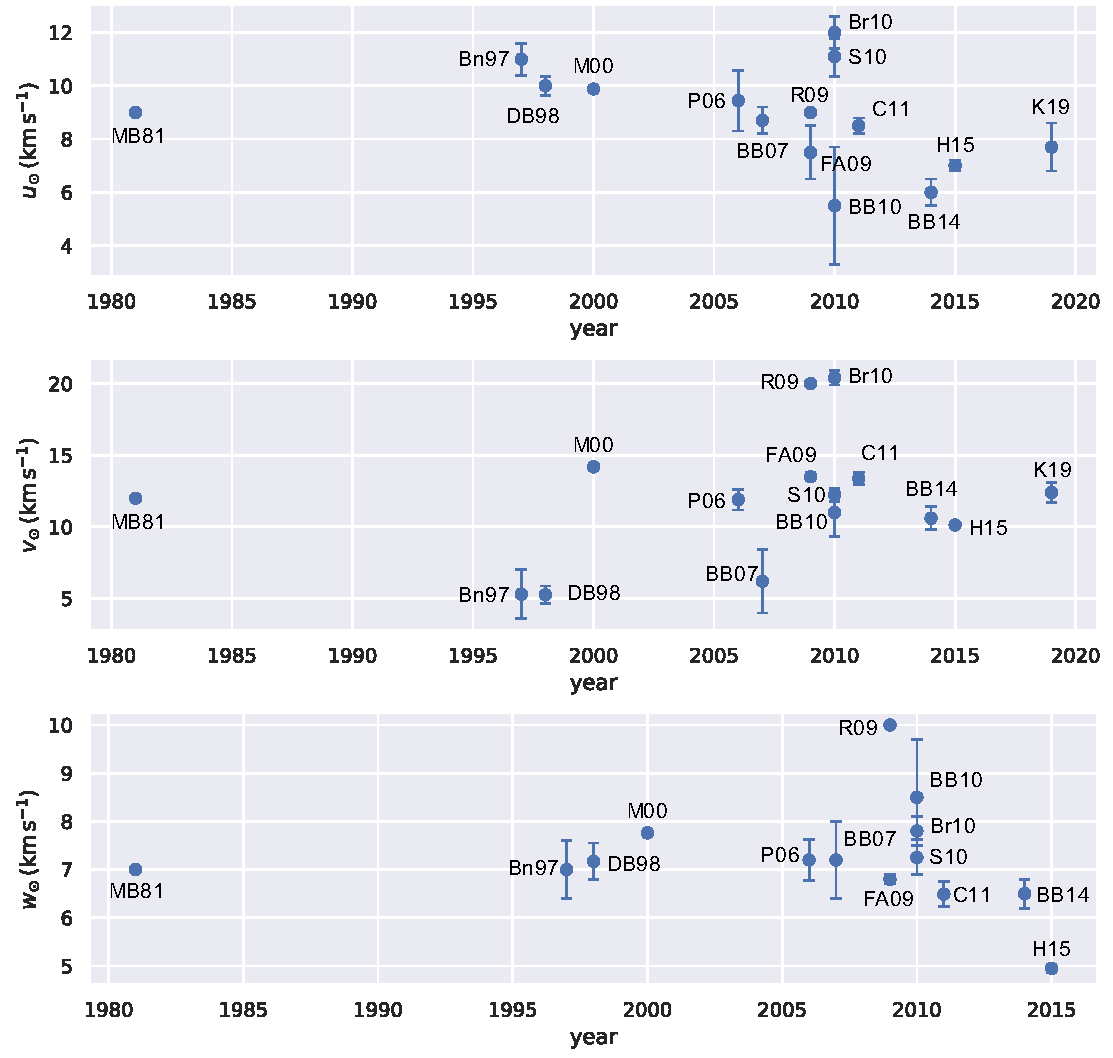
\includegraphics[width=13cm]{fig/UVW.pdf}
	\caption{先行研究の太陽運動の値のプロット。ラベルについては表\ref{table2}を参照。}
	\label{fig:uvw}
\end{figure*}